\documentclass{tufte-handout}

\title{Continuous Probabilistic Programming\thanks{CS7470 Fall 2023: Foundations of Probabilistic Programming.}}


\author[]{Steven Holtzen\\s.holtzen@northeastern.edu}

%\geometry{showframe} % display margins for debugging page layout
\setcounter{secnumdepth}{1}

\usepackage{graphicx} % allow embedded images
  \setkeys{Gin}{width=\linewidth,totalheight=\textheight,keepaspectratio}
  \graphicspath{{graphics/}} % set of paths to search for images
\usepackage{amsmath,amssymb,amsthm}  % extended mathematics
\usepackage{booktabs} % book-quality tables
\usepackage{units}    % non-stacked fractions and better unit spacing
\usepackage{multicol} % multiple column layout facilities
\usepackage{lipsum}   % filler text
\usepackage{fancyvrb} % extended verbatim environments
  \fvset{fontsize=\normalsize}% default font size for fancy-verbatim environments
\usepackage{listings}
\usepackage{tikz}
\usepackage{mathpartir}
\usepackage{subcaption}
\usepackage{mdframed}
\usepackage{epigraph}
\usepackage{enumitem}
\usepackage{stmaryrd}

\usetikzlibrary{shapes.geometric}


\usepackage[ruled,linesnumbered]{algorithm2e}
\SetKwComment{Comment}{/* }{ */}
\newcommand{\indep}{\perp \!\!\! \perp}

\tikzset{
  treenode/.style = {shape=rectangle, rounded corners,
                     draw, align=center,
                     },
  root/.style     = {treenode, font=\Large, bottom color=red!30},
  env/.style      = {treenode, font=\ttfamily\normalsize},
  dummy/.style    = {circle,draw}
}

% tikz
\usetikzlibrary{patterns,calc,backgrounds}


% TIKZ
\tikzstyle{nnf}=[
  >=stealth,font=\small,auto,scale=0.7,every node/.style={scale=0.7}
]
\tikzstyle{extnode}=[
  draw,circle,inner sep=2pt,fill=white
]

\tikzstyle{leafnode}=[
  draw,fill=gray!20,inner sep=3.5pt
]
\tikzstyle{constnode}=[
  draw,fill=white,inner sep=3.5pt
]
\tikzstyle{label}=[
  fill=white,inner sep=2.5pt
]

\tikzstyle{acarrow}=[
    decoration={markings,mark=at position 1 with {\arrow[scale=0.6]{>}}},
    postaction={decorate},
    shorten >=0.4pt,
    >=latex,
    line width=0.1
]

\tikzstyle{bnarrow}=[
    decoration={markings,mark=at position 1 with {\arrow[scale=1.5]{>}}},
    postaction={decorate},
    shorten >=0.7pt,
    >=latex,
    line width=0.3
]
\tikzstyle{bayesnet}=[
  >=latex, thick, auto
]
\tikzstyle{bnnode}=[
  draw,ellipse,minimum size=7mm,inner sep=1pt,font=\small
]
\tikzstyle{cpt}=[
  font=\footnotesize
]

\tikzstyle{graph}=[
  >=stealth,font=\small,auto,scale=1,every node/.style={scale=1}
]
\tikzstyle{node}=[
  draw,circle,inner sep=3pt,fill=white
]

% BDDs

\tikzstyle{bdd}=[
  >=latex, thick, >=stealth, font=\small,auto,scale=0.9,every node/.style={scale=0.9}
]
\tikzstyle{bddnode}=[
  draw,circle,inner sep=0pt,fill=white,minimum size=5.5mm
]

\tikzstyle{bddtriangle}=[
  draw, regular polygon, regular polygon sides = 3,inner sep=1pt,fill=white,minimum size=5.5mm
]

\tikzstyle{highedge}=[
    line width=0.9
]
\tikzstyle{lowedge}=[
    line width=0.9,dotted
]
\tikzstyle{bddterminal}=[
  draw,fill=gray!20,inner sep=2.5pt, font=\small
]

\lstdefinestyle{compact}{
  \ttfamily\tiny
}


\usetikzlibrary{positioning}

\newtheorem{theorem}{Theorem}
\newtheorem{definition}{Definition}
\newtheorem{conjecture}{Conjecture}
\newtheorem{lemma}{Lemma}
\newtheorem{exercise}{Exercise}
\newtheorem{remark}{Remark}


\usepackage{xcolor}

\definecolor{codegreen}{rgb}{0,0.6,0}
\definecolor{codegray}{rgb}{0.5,0.5,0.5}
\definecolor{codepurple}{rgb}{0.58,0,0.82}
\definecolor{backcolour}{rgb}{0.95,0.95,0.92}

\lstdefinestyle{mystyle}{
    backgroundcolor=\color{backcolour},   
    commentstyle=\color{codegreen},
    keywordstyle=\color{magenta},
    numberstyle=\tiny\color{codegray},
    stringstyle=\color{codepurple},
    basicstyle=\ttfamily\footnotesize,
    breakatwhitespace=false,         
    breaklines=true,                 
    captionpos=b,                    
    keepspaces=true,                 
    numbers=left,                    
    numbersep=5pt,                  
    showspaces=false,                
    showstringspaces=false,
    showtabs=false,                  
    tabsize=2
}

\lstset{style=mystyle}

\newcommand{\defn}[1]{\textbf{#1}}
\newcommand{\dbracket}[1]{\left \llbracket {#1} \right \rrbracket}
\newcommand{\dist}[1]{\mathtt{Dist}(#1)}
\newcommand{\true}[0]{\texttt{true}}
\newcommand{\te}[0]{\texttt{e}}
\newcommand{\false}[0]{\texttt{false}}
\newcommand{\real}[0]{\mathbb{R}}
\newcommand{\rational}[0]{\mathbb{Q}}
\newcommand{\lebesgue}[0]{\mathbb{L}}
\newcommand{\eval}[0]{\mathrm{ev}}
\newcommand{\disc}[0]{\textsc{Disc}}
\newcommand{\borel}[0]{\mathcal{B}}
\newcommand{\ent}[0]{\mathbb{S}}
\newcommand{\prog}[0]{\texttt{p}}
\newcommand{\bool}[0]{\mathbb{B}}
\newcommand{\cont}[0]{\textsc{Cont}}
\newcommand{\prop}[0]{\textsc{Prop}}
\newcommand{\bdd}[0]{\textsc{Bdd}}
\newcommand{\robdd}[0]{\textsc{Robdd}}
\newcommand{\compiles}[0]{\rightsquigarrow}

\newcommand{\bddtriangle}[1]{
    \begin{tikzpicture}
    \node [bddtriangle] {#1};
    \end{tikzpicture}}
\newcommand{\bddtrue}[0]{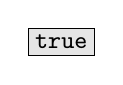
\begin{tikzpicture}
      \node [bddterminal] {$\true$};
    \end{tikzpicture}}
\newcommand{\bddfalse}[0]{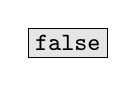
\begin{tikzpicture}
      \node [bddterminal] {$\false$};
    \end{tikzpicture}}


% Standardize command font styles and environments
\newcommand{\doccmd}[1]{\texttt{\textbackslash#1}}% command name -- adds backslash automatically
\newcommand{\docopt}[1]{\ensuremath{\langle}\textrm{\textit{#1}}\ensuremath{\rangle}}% optional command argument
\newcommand{\docarg}[1]{\textrm{\textit{#1}}}% (required) command argument
\newcommand{\docenv}[1]{\textsf{#1}}% environment name
\newcommand{\docpkg}[1]{\texttt{#1}}% package name
\newcommand{\doccls}[1]{\texttt{#1}}% document class name
\newcommand{\docclsopt}[1]{\texttt{#1}}% document class option name
\newenvironment{docspec}{\begin{quote}\noindent}{\end{quote}}% command specification environment



\begin{document}
\maketitle% this prints the handout title, author, and date

Some logistics:
\begin{itemize}
  \item Friday Oct. 20 is Systems day: Please sign up to give a presentation on a 
  system, and be sure to post your slides ahead of time in the Slack
  \item I will release and adjust the deadline for the continuous language this
  weekend based on what we've covered. It should be a pretty simple project.
  \item We will begin reading papers next week. See the instructions and 
  consult the syllabus for which papers to read.
\end{itemize}

\section{\cont{}: A tiny continuous PPL}
Syntax: 
\begin{lstlisting}[mathescape = true]
v ::= real | bool
$\tau$ ::= $\bool$ | $\real$ | $\dist{\real}$
e ::= unif | x $\leftarrow$ e | x | v | e + e | e < e | e $\lor$ e | e $\land$ e | $\neg$ e
\end{lstlisting}

\begin{itemize}
  \item As usual, our recipe will have two parts: new denotation, new
  operational semantics. We begin with denotation.

  \item \textbf{Goal}: give a denotation for \cont{} that maps terms to
  probability distributions

  \item The \texttt{unif} keyword denotes a \emph{uniform probability
  distribution on the interval} $[0,1]$. This means we need to be able to handle
  probability distributions on the interval. 

  \item For example, we can write the following program:
\begin{lstlisting}[mathescape=true]
x $\leftarrow$ unif;
return x < 1/2
\end{lstlisting}
How should we interpret this program? Intuitively, this program should 
return a distribution:
\begin{align*}
  [\true \mapsto 1/2, \false \mapsto 1/2]
\end{align*}

\item What about this more interesting program:
\begin{lstlisting}[mathescape=true]
x $\leftarrow$ unif;
y $\leftarrow$ unif;
return x + y < 1/2
\end{lstlisting}

This is significantly more challenging! The probability that this returns 
$\true$ is equal to the area of this triangle:

\begin{center}
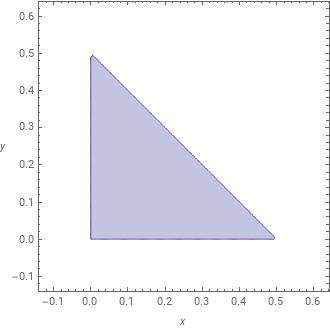
\includegraphics[width=200px]{ineq-plot.png}
\end{center}

Put differently, it is an integral:
\begin{align}
  \int_0^1 \int_0^1 \mathbb{1}(x + y < 1/2)~\mathrm{d}x~\mathrm{d}y = 1/8
\end{align}

\end{itemize}


\subsection{Probability distributions on the interval}
\marginnote{For an excellent discussion on the development of this section,
 see \citet{axler2020measure}.}
\begin{itemize}
  \item \textbf{Goal}: Define a probability distribution on the sample space
  $\Omega = [0,1]$

  \item Recall the challenge from last time: we cannot define a distribution 
  naively on points because the probability of any particular real value $\omega
  \in \Omega$ should be 0.\sidenote{Why is this the case? Assume that there is a
  probability distribution $\mu : \Omega \rightarrow [0,1]$ that assigns a 
  non-zero probability to a countably-infinite set of points in $\omega \in
  \Omega$. Then, $\sum_{\omega \in \Omega} \mu(\omega) = \infty$, which is a 
  contradiction.}

  \item Hence, we need to consider a subset of well-behaved semi-algebra of
  events on which to define a probability measure. A standard choice are the
  \emph{collection of all open intervals} contained in $[0,1]$:
  \begin{align*}
    \mathcal{J} = \{(l, u) \mid 0 \le l < u \le 1 \} \cup \{\emptyset, \Omega\}
  \end{align*}
  Why is this a good choice of events? Because we know a good way to define their 
  probability:
  \begin{align}
    \mu((l, u)) = u - l \qquad \mu(\emptyset) = 0 \qquad \mu(\Omega) = 1
    \label{eq:lebesgue}
  \end{align}

  \item The \defn{Borel $\sigma$-algebra} is the smallest $\sigma$-algebra that contains
  $\mathcal{J}$. We denote the Borel $\sigma$-algebra as $\mathcal{B}$.\sidenote{See Definition 2.27 of \citet{axler2020measure} for a discussion 
  of why the notion of a smallest $\sigma$-algebra is well-founded.} 

  \item The unique probability measure $\lambda: \borel \rightarrow [0,1]$ given
  by the extension of Eq.~(\ref{eq:lebesgue}) to $\mathcal{B}$ is called the
  \defn{Lebesgue measure} on the interval. For example:
  \begin{align*}
    \lambda\left((0, \frac{1}{2}) \cup (\frac{3}{4}, 1) \right) = 1/2 + 1/4 = 3/4.
  \end{align*}
  


  \item Now we will need a new generalized notion of random variable for this new 
  setting. A random variable will be defined as a well-behaved function out of 
  the sample space:
  \begin{definition}[Measurable function]
    Let $(\Omega, \calF, \mu)$ be a probability space, $(X, \mathcal{A})$ be 
    a measurable space, and $f : \Omega \rightarrow X$ 
    be a function. The function $f$ is called \emph{measurable} if, 
    for any $A \in \mathcal{A}$, it is the case that $f^{-1}(A) \in \calF$.
  \end{definition}

  Measurable functions $f : [0,1] \rightarrow \real$ defined on $([0,1], \borel,
  \lambda)$ are often called \emph{Borel-measurable}. Most functions you have
  seen are Borel-measurable.\sidenote{For instance, all continuous functions are
  Borel measurable.}

  \item Measurable functions behave like random variables in that they induce 
  probability measures on their co-domains via a \emph{push-forward}:
  \begin{definition}
    Let $(\Omega, \calF, \mu)$ be a probability space, $(X, \mathcal{A})$ be a 
    measurable space, and $f: \Omega \rightarrow X$ 
    be a measurable variable. Then, the \emph{push-forward probability measure}
    $\nu : \mathcal{A} \rightarrow [0,1]$ is defined:
    \begin{align}
      \nu(A) = \mu(f^{-1}(A)).
    \end{align}
  \end{definition}

\end{itemize}

\section{Denotation of \cont{}}

\begin{itemize}
  \item These semantics are in the style of \emph{Markov kernels}~\citep{kozen1979semantics,barthe2020foundations}
  % \item Three kinds of semantics:\sidenote{
  %   Recall that we define $\dbracket{\Gamma}$ as the collection of 
  %   all substitutions that are compatible with $\Gamma$.
  %   For example, if we have $\Gamma = \{x : \bool\}$, we may have the 
  %   substitution $[x \mapsto \true]$ in $\dbracket{\Gamma}$.
  % }
  % \begin{itemize}
  %   \item For terms $\Gamma \vdash \te : \dist{\real}$, we have that
  %   $\dbracket{\Gamma \vdash \te : \dist{\real}} : \dbracket{\Gamma} \rightarrow
  %   \borel \rightarrow [0,1]$ yields a probability measure on the Borel sets

  %   \item For pure terms $\Gamma \vdash \te : \real$, denotation yields a 
  %   measurable function: $\dbracket{\Gamma \vdash \te : \real} :
  %   \dbracket{\Gamma} \rightarrow \real$; similar for terms of type $\bool$.
  % \end{itemize}

  \item The case for pure terms is relatively simple
  \item \marginnote{The semantics of $x \leftarrow \te_1; \te_2$ is the bind operator 
  for the Giry monad~\citep{giry2006categorical,ramsey2002stochastic}. 
  This definition involves a \emph{generalized integral} wrt. a base measure. 
  }
  First we give the semantics:
  \begin{fullwidth}
  \begin{align*}
    \dbracket{\texttt{unif} : \dist{\real}}(A) &= \lambda(A) \\
    \dbracket{\texttt{return}~\te : \dist{\real}}(A) &= \mathbb{1}(\dbracket{\te} \in A) = \delta_{\dbracket{\te}}\\
    \dbracket{x \leftarrow \te_1; \te_2}(A) &= \E_{v \sim \dbracket{\te_1}} \Big[\dbracket{\te_2[v/x]}\Big] = \int_\real \dbracket{\te_2[v/x]}(A) ~\rmd \dbracket{\te_1}(v)
  \end{align*}
\end{fullwidth}
The \emph{Diract-delta} $\delta_v(A)$ denotes a distribution that assigns a
probability of 1 to any event that contains $v \in \Omega$.
  \item Integration wrt. the Lebesgue base measure is written 
  $\int f(x) ~ \rmd \lambda(x)$. It behaves just like Riemann integration (integrals from 
  high school) if $f$ is a suitably well-behaved function (i.e., continuous). 
  \item Example:
\begin{fullwidth}
  \begin{align*}
    \dbracket{x \leftarrow \texttt{unif}; \texttt{return}~x+x}((0, 1/2)) &= 
    \int_0^1 \dbracket{\texttt{return}~v + v}(v)((0, 1/2)) ~ \rmd \lambda(v) \\
    &= \int_0^1 \mathbb{1}(v + v \in (0, 1/2)) ~ \rmd \lambda(v) \\
    &= \int_0^{1/4} 1~\rmd \lambda(v) \\
    &= 1/4
  \end{align*}
\end{fullwidth}
\item Integration wrt. the Dirac measure $\delta_v$ is defined: 
\begin{align}
  \int_\real f(x) ~ \rmd \delta_v(x) \triangleq f(v).
\end{align}
This lets us interpret programs with \texttt{return}:
\begin{align*}
  \dbracket{x \leftarrow \texttt{return}~1; \texttt{return}~x+x}(A) &= 
  \int_\real \dbracket{\texttt{return}~v+v}(A)~\rmd \delta_1(v) \\ 
  &= \int_\real \delta_{v+v}(A)~\rmd \delta_1(v) \\
  &= \delta_{2}(A).
\end{align*}
\end{itemize}

\section{Sampling semantics for \cont{}}
\begin{itemize}
  \item These are very similar the sampling semantics for \disc{} from last time,
  except we need a different source of random bits 
  \item We will entropy $\sigma \in [0,1]^\nat$, i.e. $\sigma$ is a countably infinite
  stream of real values drawn from the interval. We again define $\pi_L$ and $\pi_R$ 
  as ways of splitting the entropy into independent sets.
  \item Then we will define a big-step relation $\sigma \vdash \te \Downarrow v$:
  \begin{mathpar}
    \inferrule{}{v :: \sigma \vdash \texttt{unif} \Downarrow v}
    \and
    \inferrule{\pi_L(\sigma) \vdash \te_1 \Downarrow v_1 \and 
    \pi_R(\sigma) \vdash \te_2[v_1/x] \Downarrow v_2 }
    {\sigma \vdash x \leftarrow \te_1; \te_2 \Downarrow v_2}
    \and
    \inferrule{}{\sigma \vdash \texttt{return v} \Downarrow v}
  \end{mathpar}
\end{itemize}

\begin{theorem}
  Assume $\te$ is a well-typed closed term and $\Pr$ is the 
  distribution on the entropy space. Then, for any 
  event $A \in \borel$, we have that: 
  \begin{align} 
    \E_{\sigma \sim \Pr} \Big[\mathbb{1}[eval(\te, \sigma) \in A] \Big] = 
    \dbracket{\te}(A).
  \end{align}
\end{theorem}

\section{Continuous observation}

Add a new \texttt{observe} keyword to \cont{}:

\begin{lstlisting}[mathescape = true]
v ::= real | bool
$\tau$ ::= $\bool$ | $\real$ | $\dist{\real}$
e ::= unif | x $\leftarrow$ e | x | v | e + e | e * e | e < e | e $\lor$ e | e $\land$ e | $\neg$ e 
   | observe e; e
\end{lstlisting}

This keyword is surprisingly powerful. Suppose we want to infer something 
about the distribution of people's heights. Suppose we assume that people 
are between 65 and 73 inches tall, and that people 
vary from the true value by 1 inch.
Then, we observe that someone's height 
is between 71 and 73 inches, 
and want to update prior beliefs about how people's heights are distributed.
We can model this as the following program:

\begin{lstlisting}[mathescape=true]
h $\leftarrow$ unif;
height_dist $\leftarrow$ (h * 4) + 69
eps1 $\leftarrow$ unif;
observe 71 < height_dist + eps1 < 73;
return height_dist
\end{lstlisting}

\bibliographystyle{plainnat}
\bibliography{../bib}


\end{document}